\documentclass[handout]{beamer}
\usepackage[export]{adjustbox}
\usepackage[frenchb]{babel}
\usepackage[T1]{fontenc}
\usepackage[utf8]{inputenc}
\usepackage{listings}
\usepackage{eurosym}
\usepackage{fancyvrb}
\usepackage{textpos}
\usetheme{Warsaw}
\usepackage{eso-pic}

\title[Linux Embarqué, INSA Rouen]{Découverte de Linux Embarqué}
\author{maxime.chevallier@smile.fr}
\date{09 septembre 2016}
\institute{Smile / Open Wide Ingénierie}
\begin{document}

% Afficher plan à chaque section
\AtBeginSection[]{
	\begin{frame}
		\tableofcontents[currentsection, hideallsubsections]
	\end{frame}
}
\beamertemplatenavigationsymbolsempty{} % /o\ Pas de symboles de nav

% Numeros de slides
\addtobeamertemplate{navigation symbols}{}{%
    \usebeamerfont{footline}%
    \usebeamercolor[fg]{footline}%
    \hspace{1em}%
    \insertframenumber/\inserttotalframenumber
}

\newcommand\AtPagemyUpperLeft[1]{\AtPageLowerLeft{%
\put(\LenToUnit{0.8\paperwidth},\LenToUnit{0.9\paperheight}){#1}}}
\AddToShipoutPictureFG{
	  \AtPagemyUpperLeft{{\includegraphics[width=2cm,keepaspectratio]{img/owi-smile.png}}}
  }%


\setbeamercolor{footline}{fg=blue}
\setbeamerfont{footline}{series=\bfseries}
\setbeamertemplate{caption}{\raggedright\insertcaption\par}
\setbeamerfont{caption}{size=\tiny}
    \begin{frame}

	\titlepage

	\includegraphics[width=3cm]{img/owi-smile.png}
    \end{frame}

\begin{frame}
\tableofcontents
\end{frame}

\section{Système embarqué}
\begin{frame}[t]
	\center{\huge{Système embarqué}}
	\begin{columns}
	\begin{column}[t]{0.30\linewidth}
		\begin{figure}
			\includegraphics<2->[height=2.5cm]{img/roomba.jpg}
			\uncover<2->{\caption{aspirateur du futur}}
		\end{figure}
	\end{column}
	\begin{column}[t]{0.30\linewidth}
		\begin{figure}
			\includegraphics<3->[height=2.5cm]{img/tesla.jpg}
			\uncover<3->{\caption{voiture du futur}}
		\end{figure}
	\end{column}
		\begin{column}[t]{0.30\linewidth}
		\begin{figure}
			\includegraphics<4->[height=2.5cm]{img/router.jpg}
			\uncover<4->{\caption{routeur normal}}
		\end{figure}
	\end{column}
	\end{columns}
	\uncover<5->{\center{Systèmes embarqués :)}}
\end{frame}

\begin{frame}[t]
	\center{\huge{Système embarqué}}
	\begin{columns}
	\begin{column}[t]{0.45\linewidth}
		\begin{figure}
			\includegraphics<2->[height=2.5cm]{img/raspi.jpg}
			\uncover<2->{\caption{Raspberry pi 2}}
		\end{figure}
	\end{column}
	\begin{column}[t]{0.45\linewidth}
		\begin{figure}
			\includegraphics<3->[height=2.5cm]{img/arduino.jpg}
			\uncover<3->{\caption{Arduino UNO}}
		\end{figure}
	\end{column}
	\end{columns}
	\uncover<4->{\center{Pas des systèmes embarqués :(}}
\end{frame}

% C'est quoi ?
\subsection{Contraintes}
\begin{frame}[t]
	\center{\huge{Contraintes}}
	\begin{block}<1->{Coûts matériels}
		\begin{itemize}
			\item Processeur
			\item Mémoire(s)
			\item Périphériques
		\end{itemize}
	\end{block}
	\begin{block}<2->{Coûts logiciels}
		\begin{itemize}
			\item Licenses ?
			\item Développements spécifiques ?
			\item Expertise ou support externe ?
			\item Evolution du produit ?
		\end{itemize}
	\end{block}
\end{frame}

\begin{frame}[t]
	\center{\huge{Contraintes}}
	\begin{block}{Performances}
		\begin{itemize}
			\item Latences : Temps réel
			\item Temps de boot
			\item Capacité de calcul
		\end{itemize}
	\end{block}
	\begin{block}<2->{Environnement}
		\begin{itemize}
			\item Durabilité
			\item Environnement physique hostile
			\item Consommation
			\item Normes ( Radio, GPS )
		\end{itemize}
	\end{block}
\end{frame}

\begin{frame}[t]
	\begin{block}<1->{Microcontrôleur}
		\begin{columns}[t]
			\begin{column}[T]{0.25\textwidth}
				\begin{figure}
					\includegraphics<1->[width=2.2cm]{img/atmega.jpg}
					\uncover<1->{\caption{Atmel ATMega 328}}
				\end{figure}
			\end{column}
			\begin{column}{0.70\textwidth}
				\begin{itemize}
					\item<2-> 1\euro50 / pièce
					\item<2-> 1 Cœur AVR 8bits @ 20 MHz
					\item<2-> 2 Ko RAM, 32 Ko Progmem
					\item<2-> I2C, SPI, UART
				\end{itemize}
			\end{column}
		\end{columns}
	\end{block}
	\begin{block}<3->{Microprocesseur}
		\begin{columns}[t]
			\begin{column}[T]{0.25\textwidth}
				\begin{figure}
					\includegraphics<3->[width=2.5cm]{img/imx.jpg}
					\uncover<3->{\caption{NXP iMX6 Quad}}
				\end{figure}
			\end{column}
			\begin{column}{0.70\textwidth}
				\begin{itemize}
					\item<4-> 36\euro / pièce
					\item<4-> 4 Cœurs ARM 32 bits @ 1GHz
					\item<4-> 256 Ko RAM, 96 Ko boot ROM
					\item<4-> DDR3, SDIO, eth, USB, HDMI, PCIe\dots
				\end{itemize}
			\end{column}
		\end{columns}
	\end{block}
\end{frame}


\begin{frame}
	\center{\huge{OS Temps-réel libres}}
	\begin{block}<2->{Contiki}
		\begin{columns}
		\begin{column}{0.50\textwidth}
		\begin{itemize}
			\item Orienté Networking et IoT
			\item Petite emprunte mémoire
			\item Riche en fonctionnalités
		\end{itemize}
		\end{column}
		\begin{column}{0.30\textwidth}
			\includegraphics[height=2cm]{img/amp.jpg}
		\end{column}
		\end{columns}
	\end{block}
	\begin{block}<3->{freeRTOS}
		\begin{columns}
			\begin{column}{0.50\textwidth}
				\begin{itemize}
					\item Petite emprunte mémoire
					\item Beaucoup d'architectures
					\item Éprouvé dans l'industrie
				\end{itemize}
			\end{column}
			\begin{column}{0.20\textwidth}
				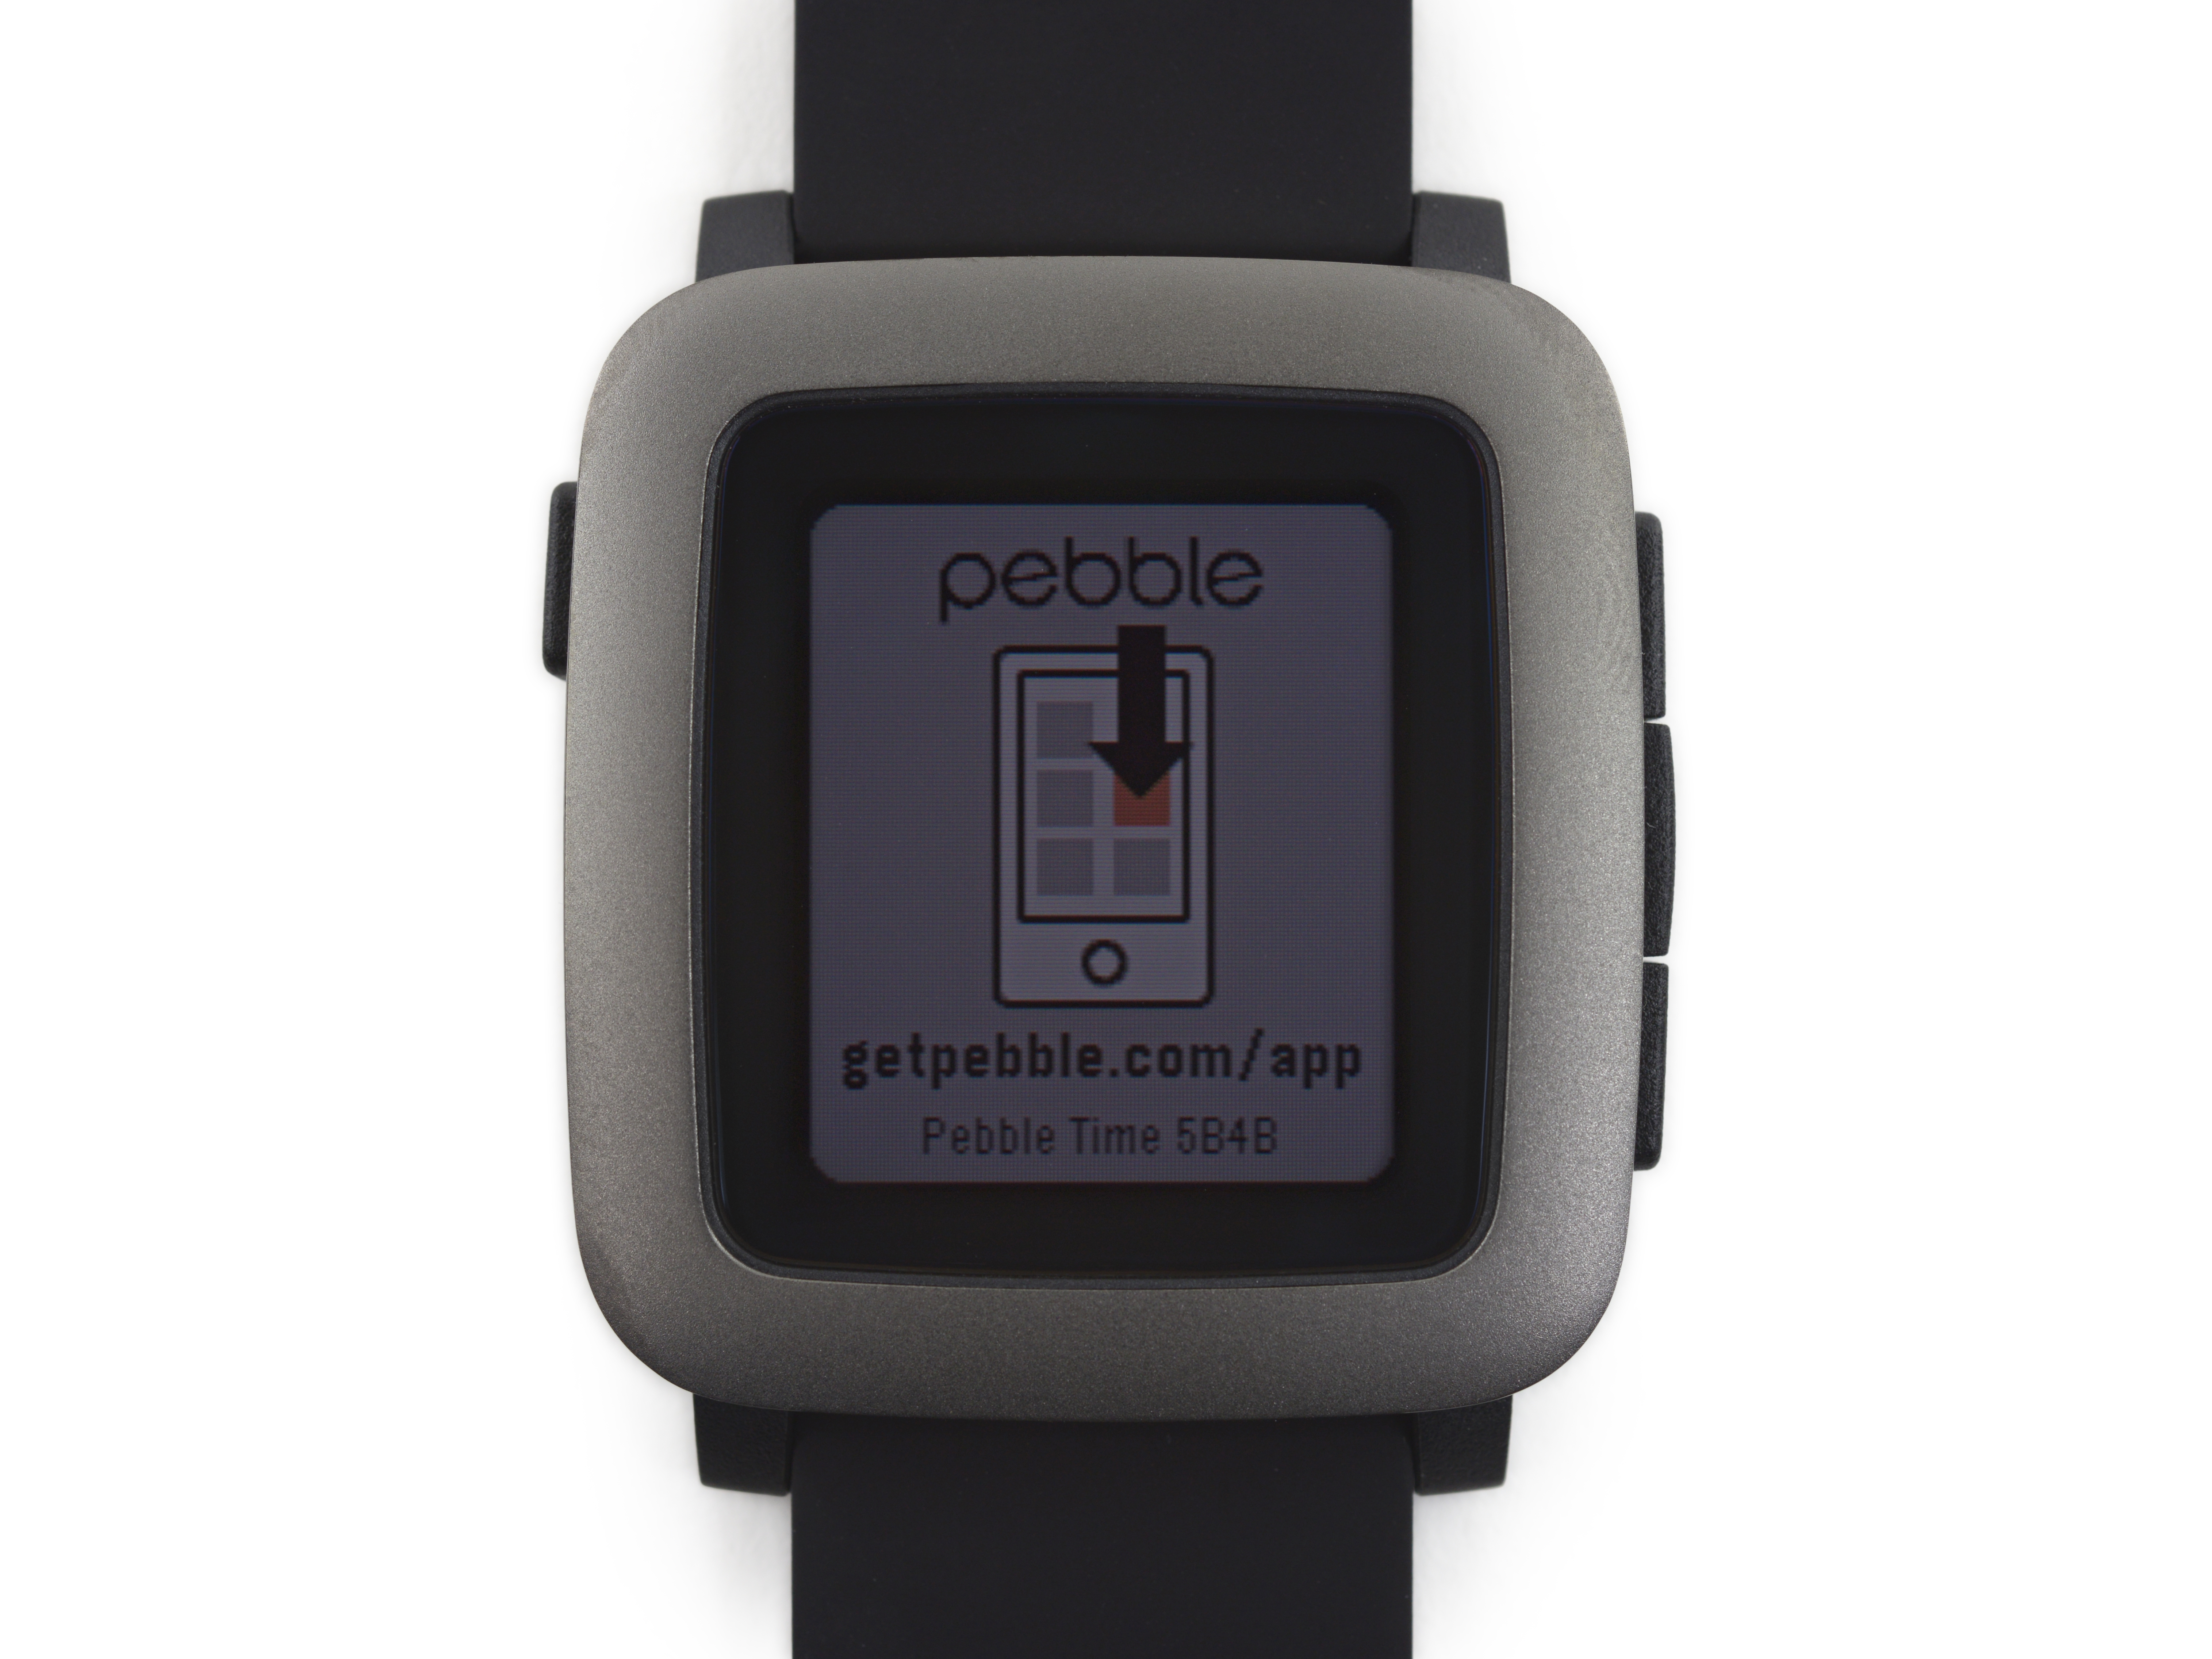
\includegraphics[height=2cm]{img/pt.jpg}
			\end{column}
			\begin{column}{0.20\textwidth}
				\includegraphics[height=2cm]{img/cubesat.jpg}
			\end{column}
		\end{columns}
	\end{block}
\end{frame}


% schéma
\section{Kernel}
\begin{frame}
	\center{\huge{Noyau}}
	\begin{columns}
	\begin{column}{0.38\linewidth}
		\begin{figure}
			\includegraphics[height=2.5cm]{img/arch_linux_full.png}
			 \caption{kernel}
		\end{figure}
	\end{column}
	\begin{column}{0.60\linewidth}
		\begin{itemize}
			\item<2-> Gère le matériel
			\item<3-> Gère les ressources
			\item<4-> Implémente certains protocoles
			\item<5-> Couche d'abstraction
			\item<6-> Isolé de l'espace utilisateur
			\item<7-> Composant critique
		\end{itemize}
	\end{column}
	\end{columns}
\end{frame}


\begin{frame}
	\center{\huge{Linux}}
	\begin{columns}[t]
		\begin{column}{0.70\textwidth}
			\begin{itemize}
				\item<2-> Beaucoup d'architectures
				\item<3-> Beaucoup de périphériques
				\item<4-> Beaucoup de fonctionnalités
				\item<5-> Communauté active
				\item<6-> Entièrement configurable
				\item<7-> Libre
			\end{itemize}
		\end{column}
		\begin{column}{0.25\textwidth}
			\begin{figure}
				\includegraphics[height=2cm]{img/tux.png}
				\caption{Tux}
			\end{figure}
		\end{column}
	\end{columns}
	\begin{block}<8->{Variantes}
		\begin{itemize}
			\item<8-> Temps réel : Preempt-RT, xenomai
			\item<9-> Microcontrolleur : uCLinux
			\item<10-> Sécurité : SELinux, grsecurity
		\end{itemize}
	\end{block}
\end{frame}
% choix de la version
\subsection{Drivers}
\begin{frame}
	\center{\huge{Drivers}}
	\begin{itemize}
		\item Support d'un périphérique
		\item Support d'un protocole
		\item Libre ou Propriétaire
	\end{itemize}
	\begin{block}<2->{Kernel module}
		\begin{itemize}
		\item Extension du kernel
		\item Intégration statique ou dynamique
		\item \textbf{Lié à une version du kernel}
		\item Gestion des dépendances
		\end{itemize}
	\end{block}
\end{frame}
% drivers, support
\subsection{Configuration}
\begin{frame}[t]
	\center{\huge{Configuration du noyau}}
	\begin{columns}[T]
		\begin{column}{0.50\textwidth}
		\begin{itemize}
			\item Choix des drivers
			\item Choix des fonctionnalités
			\item Options de debug
			\item Options d'optimisation
		\end{itemize}
		\end{column}
		\begin{column}{0.48\textwidth}
			\vspace{-0.2cm}
			\begin{figure}
				\includegraphics<2->[height=3cm]{img/menuconfig.png}
			\end{figure}
		\end{column}
	\end{columns}
	\begin{block}<2->{Kconfig}
		\begin{itemize}
			\item Plusieurs UI
			\item Dépendances entre options
			\item Génère un fichier de conf
		\end{itemize}
	\end{block}
\end{frame}
% choix des options : selon matos, contraintes

% Schema
\section{Userspace}
	\begin{frame}
		\begin{figure}
		\includegraphics[height=4cm]{img/arch_linux_full.png}
		\caption{kernel + userspace}
		\end{figure}
	\end{frame}
	\begin{frame}
		\center{\huge{Système d'init}}
		\begin{itemize}
			\item Premier processus lancé
			\item Lance les autres processus
			\item Influe sur le temps de boot
		\end{itemize}
		\begin{block}{SysV init}
			\begin{itemize}
				\item Scripts
				\item Peu de parallélisation
			\end{itemize}
		\end{block}
		\begin{block}{Systemd}
			\begin{itemize}
				\item Fichiers de configuration
				\item Parallélisation et dépendances
				\item Plus complexe
			\end{itemize}
		\end{block}
	\end{frame}

	\begin{frame}
		\begin{block}{Librairies}
			\begin{itemize}
				\item libC : GNU libC, uClibC, dietlibC
				\item librairies métier
			\end{itemize}
		\end{block}
		\begin{block}{Utilitaires}
			\begin{itemize}
				\item Commandes standard : GNU Coreutils, Busybox
				\item Applications métier
				\item Daemons système
			\end{itemize}
		\end{block}
	Choix dicté par les contraintes de stockage.
	\end{frame}


\section{Bootloader}
%role
\begin{frame}[t]
	%schema boot + kernel
	\begin{columns}[t, totalwidth=\textwidth]
		\begin{column}[t]{0.40\linewidth}
		\begin{figure}
			\includegraphics<1-5>[width=4cm]{img/boot_bl.png}
			\includegraphics<6>[width=4cm]{img/boot_bl_kern.png}
			\includegraphics<7->[width=4cm]{img/boot.png}
			\caption{boot sequence}
		\end{figure}

	\end{column}
		\begin{column}[t]{0.45\linewidth}
	\begin{block}{Boot Sequence}
		\begin{itemize}
			\item<1-> Power On
			\item<2-> Bootloader chargé
			\item<3-> Bootloader exécuté
			\item<4-> Init matériel
			\item<5-> Noyau chargé
			\item<6-> Noyau exécuté
			\item<7-> /sbin/init appelé
		\end{itemize}
	\end{block}
	\end{column}
	\end{columns}
\end{frame}
%U Boot
\begin{frame}
	\center{\huge{Das U-Boot}}

\end{frame}

% Barebox
\begin{frame}
	\center{\huge{Barebox}}
\end{frame}


\section{Build system}
\begin{frame}[t]
	\center{\huge{Construire son système}}
	\begin{figure}
		 \includegraphics[height=1.5cm]{img/build.png}
	\end{figure}
	\vspace{-1.1cm} % #propreté
	\begin{columns}[t]
	\begin{column}{0.45\textwidth}
	\uncover<2->{\center{Non merci !}}
	\begin{block}<3->{Distribution classique}
		\begin{itemize}
			\item Simple
			\item Pas flexible
			\item Pas optimisé
			\item Architectures classiques
		\end{itemize}
	\end{block}
	\end{column}
	\begin{column}{0.45\textwidth}
	\uncover<4->{\center{Trop facile !}}
	\begin{block}<5->{À la main}
		\begin{itemize}
			\item Flexible
			\item Pas reproductible
			\item Pas maintenable
			\item Pas de dépendances
		\end{itemize}
	\end{block}
	\end{column}
	\end{columns}
\end{frame}
\begin{frame}
	\center{\huge{Build system}}
	\begin{itemize}
		\item<1-> Configure, construit et package les composants
		\item<2-> Gère les dépendances
		\item<3-> Permet la reproductibilité
		\item<4-> Génère la chaine de cross-compilation
	\end{itemize}
\begin{block}<5->{Choix critique}
	\begin{itemize}
		\item<6-> Conditionne le développement
		\item<7-> Conditionne l'évolution du projet
		\item<8-> Conditionne les livrables
	\end{itemize}
\end{block}
\end{frame}
% schema
\subsection{Buildroot}
\begin{frame}
	\center{\huge{Buildroot}}
	\begin{columns}
		\begin{column}{0.65\textwidth}
			\begin{itemize}
				\item<1-> Makefiles, Kconfig
				\item<2-> Rootfs, Bootloader, Kernel, Toolchain
				\item<3-> Répandu et simple d'utilisation
				\item<4-> 1 carte = 1 buildroot
			\end{itemize}
		\end{column}
		\begin{column}{0.30\textwidth}
			\begin{figure}
				 \includegraphics<1->[height=2cm]{img/buildroot.png}
				 \uncover<1->{\caption{Logo buildroot}}
			\end{figure}
		\end{column}
	\end{columns}
	\begin{block}<5->{Pourquoi Buildroot ?}
		\begin{itemize}
			\item<6-> Cartes sans variantes
			\item<7-> Prototypage
			\item<8-> Projet "Simple"
		\end{itemize}
	\end{block}
\end{frame}
% buildroot
\subsection{Yocto}
% yocto
\begin{frame}
	\center{\huge{Yocto project}}
		\begin{itemize}
			\item<2-> Groupes de composants réutilisables : Layers
			\item<3-> Scripts surchargeables : Recipes
			\item<4-> Grosse base de composants
			\item<5-> Rootfs, Kernel, Bootloader, Toolchain, Paquets
			\item<6-> Difficile à prendre en main
		\end{itemize}
	\begin{block}<7->{Pourquoi Yocto ?}
	\begin{itemize}
		\item<8-> Gros projet
		\item<9-> Cartes avec variantes
		\item<10-> Favoriser la réutilisation
	\end{itemize}
	\end{block}
\end{frame}

\begin{frame}[t]
	\center{\huge{Yocto c'est simple}}
	\begin{figure}
		 \includegraphics<2->[height=5.1cm]{img/yocto.png}
		 \uncover<2->{\caption{\tiny{http://www.yoctoproject.org/docs/2.1/mega-manual/mega-manual.html}}}
	\end{figure}
\end{frame}

\begin{frame}[t]
	\center{\huge{Yocto c'est simple ( en vrai )}}
	\begin{columns}
		\begin{column}{0.45\textwidth}
			\begin{figure}
%				 \includegraphics<2>[height=3cm]{img/metas.png}
%				 \includegraphics<3>[height=3.1cm]{img/metas_zoom_1.png}
%				 \includegraphics<4>[height=3.2cm]{img/metas_zoom_2.png}
				 \includegraphics<5>[height=3cm]{img/metas_zoom_b12.png}
			\end{figure}
		\end{column}
		\begin{column}{0.55\textwidth}
			\begin{itemize}
				\item<2-> Layers : Base + custom
				\item<3-> Recipes : Comment construire un paquet ?
				\item<4-> Recipes : Possibilité d'extension
				\item<5-> Machine : Layers + Recipes
			\end{itemize}
		\end{column}
	\end{columns}
\end{frame}

\begin{frame}
	\center{\huge{Résumé}}
	\begin{itemize}
		\item<2-> Bootloader : U-Boot ( ou barebox )
		\item<3-> Kernel : Drivers, Version, Configuration
		\item<4-> Userspace : LibC, Init, packages
		\item<5-> Build system : Buildroot ou Yocto
	\end{itemize}
	\begin{block}<6->{Logiciel libre}
		\begin{itemize}
			\item Facilite le debug
			\item Facilite le développement
			\item Contrôle total sur le système
			\item Communauté en support
		\end{itemize}
	\end{block}
\end{frame}

\begin{frame}
	\center{\huge{Questions ?}}
\end{frame}
% interet du libre
% conclu


\end{document}
